\chapter{Introduction}
The problem of the transport of a solute arises in many areas of science. In
physiology, examples include the transport of nutrients from the maternal to the
foetal blood in the placenta (see figure~\ref{fig:placenta}; the exchange of oxygen
and carbon dioxide by the alvioli in the lungs (see figure~\ref{fig:alveolus}).

\begin{figure}[ht!]
    \centering
    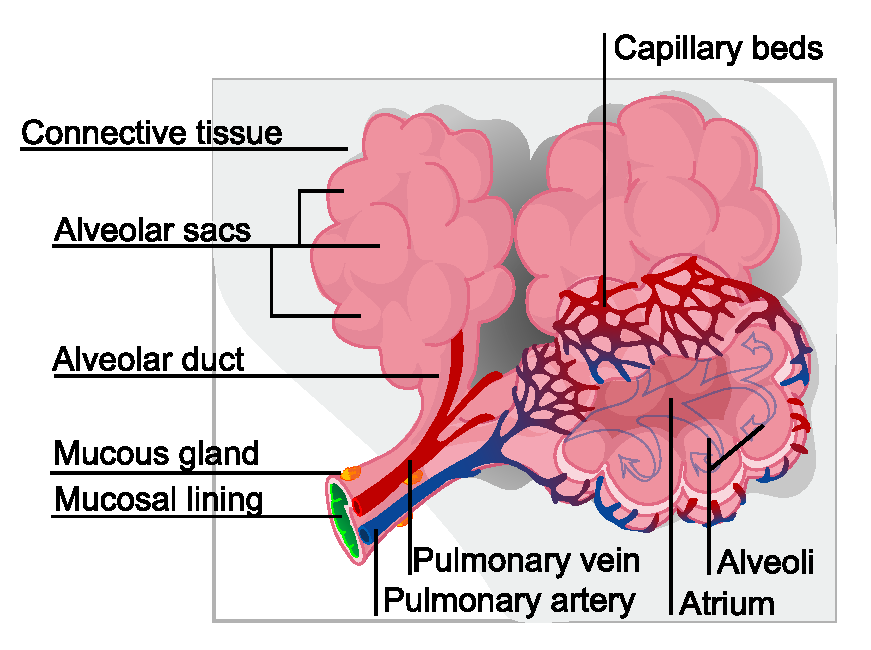
\includegraphics[width=0.7\textwidth]{introduction/figures/alveolus}
    \caption{\label{fig:alveolus}Schematic of an alveolar acini (from
http://en.wikipedia.org/wiki/File:Alveolus\_diagram.svg)}
\end{figure}
\begin{figure}[ht!]
    \centering
    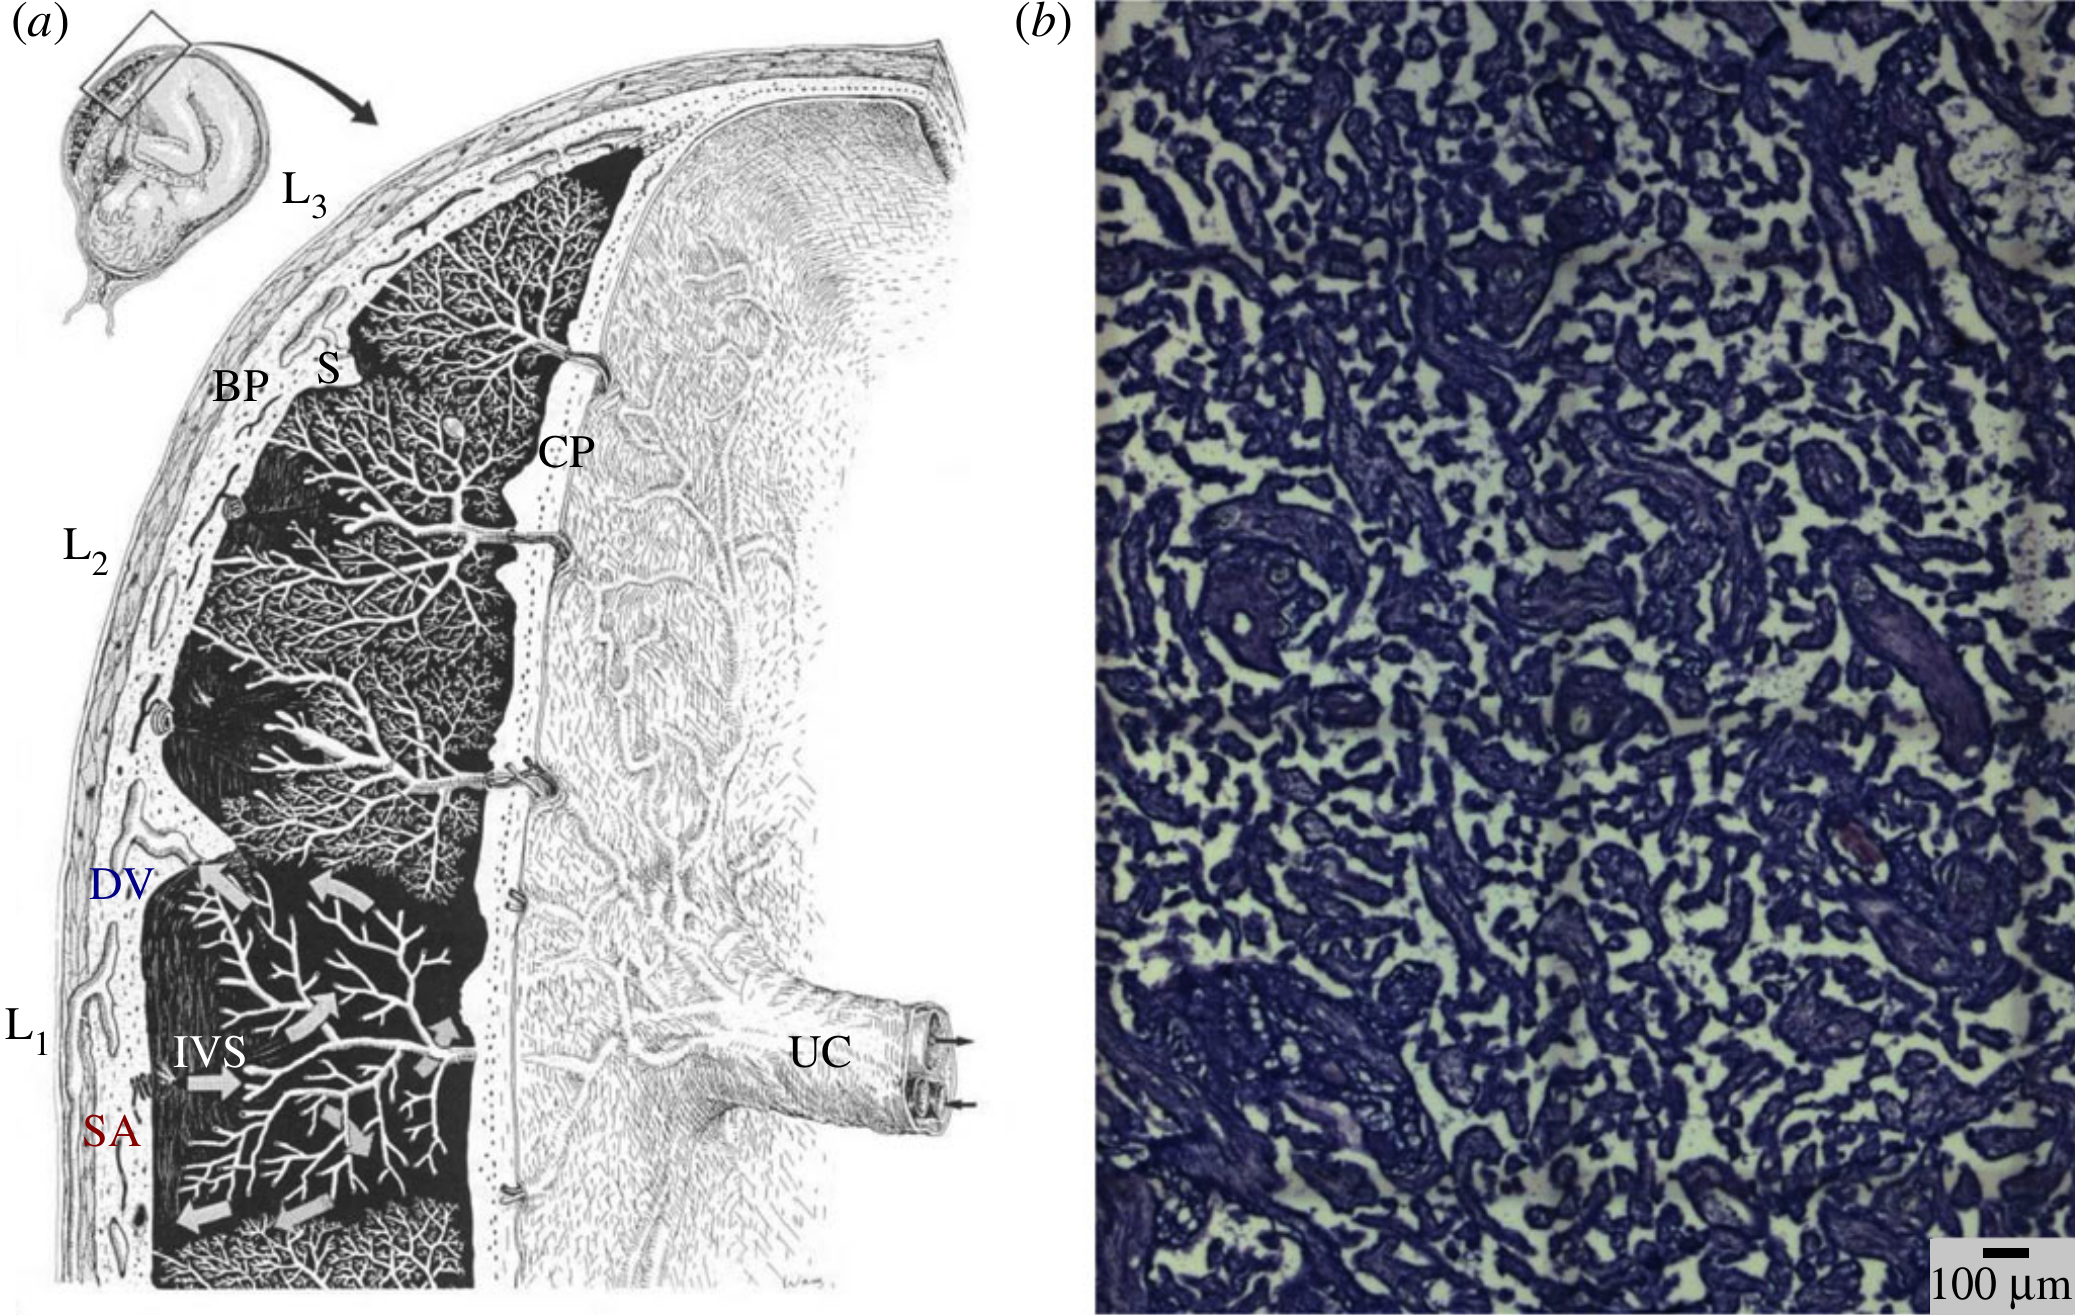
\includegraphics[width=0.7\textwidth]{introduction/figures/placentarast}
    \caption{\label{fig:placenta}Schematic of the placenta (from
    \cite{chernyavsky2012characterizing})}
\end{figure}

\todo{More examples? Other fields - earth science, industry \ldots}

We use two broad approaches to model transport phenomena: continuum models and
agent based models. The relationship between these approaches is another focus
and a goal is to provide a unified model incorporating features of both types of
model.

Both approaches assign a representation of concentration to each
spatial location. In continuum models, physical space is represented as an
interval of the real numbers and the concentration takes positive real values.
In contrast, the most basic individual based models involve finitely many
spatial locations (called ``urns'') and each urn can hold a positive integral
number of particles.

When one begins to take certain limits of the individual based system, the
distinction between the two approaches becomes less well-defined. For example,
one may obtain a continuum model from a discrete model in the appropriate limits
of a large number of urns and large numbers of particles. \todo{clarify, refs}

\section{Literature review}
\subsection{Transport phenomena in physiology and biology}
Transport phenomena are ubiquitous in physiological and biological systems and
can been seen on a vast range of time- and length-scales.

\begin{itemize}
    \item placenta
    \item lung \cite{grebenkov2005diffusion}
    \item ion channels
    \item ants (traffic)
\end{itemize}

\subsection{Individual based models}
\todo{\cite{schadschneider2010stochastic} reserve ``individual'' for
non-stochastic models, and ``population'' stochastic}

An individual based approach models a transport problem by analysing the
stochastic interactions between discrete entities in a population.
\citet{van2007stochastic} and \citet{gardiner2009stochastic} give thorough
accounts of general stochastic processes. Generally, physical space is
discretised into a finite set of locations, which we will refer to as ``urns'',
which each hold a number of particles. Different types of models are based on
the capacity of the urns and whether time is represented as a discrete or
continuous variable. For example, exclusion processes (REF) and zero range
processes REF blah.

%Applying this approach to the problem of solute transport, the entities
%represent the particles of the solute. The physical interaction of the particles
%with each other gives rise to macroscopic phenomena such as diffusion. The
%particle-scale interactions are modelled by a set of \emph{events}, which are
%problem specific. Once the microscopic properties of an individual based model
%have been specified, it is possible to create realisations of the system using a
%stochastic simulation algorithm --- for example, the Gillespie algorithm
%(described below). The model is random in nature, with the events being randomly
%selected from an appropriate probability distribution. As such, in order to find
%the statistical properties of the system, an ensemble of realisations can be
%created from which properties can be estimated. In addition to this, we can make
%theoretical predictions (in some cases, exact expressions, and in others,
%approximations) of the statistical properties of an individual based system.
%These are typically derived from a Master equation, which describes the time
%evolution of the probability distribution defining the system.

The two main types of randomness in individual based models are
\begin{itemize}
    \item Intrinsic noise --- randomness arising from the stochastic nature of the
        physical problem;
    \item Quenched disorder --- randomness of a parameter of the system which is
        usually chosen and fixed before allowing the system to evolve.
\end{itemize}
In solute transport in a disordered medium, a source of quenched disorder is the
randomness of the sink locations.
\todo{elaborate?}

We are interested in macroscopic features of the system, including their
statistics, which are expected to arise from both types of disorder and their
interactions.

\begin{itemize}
    \item General stochastic processes \cite{van2007stochastic},
        \cite{gardiner2009stochastic}
    \item General stochastic processes and specifically transport processes
        \cite{schadschneider2010stochastic}
    \item Exclusion processes
    \item Zero range processes (apparently introduced in
        \cite{spitzer1970interaction})
        \begin{itemize}
            \item There is a mapping from exclusion processes to ZRPs (under
                certain conditions)
            \item ZRPs exhibit a ``condensation transition analogous to
                Bose-Einstein condensation''
            \item It's ``known'' that ZRPs in a 1D periodic domain have a
                factorisable pdf in steady state (Schadscheider et al)
            \item Their exact steady state solution is also ``known''
                (Schadscheider et al)
            \item ``Zero-range process with open boundaries'' gives the
                open-boundaries stationary distribution (our problem)
        \end{itemize}
    \item ``Quantum formalism'' of the master equation allows analogies
        with quantum spin chains to be made
\end{itemize}

\subsubsection{Stochastic simluation}
\begin{itemize}
    \item Gillespie \cite{gillespie1976general} \cite{gillespie1977exact}
    \item Others (next reaction method etc.) \cite{anderson2007modified} gives
        summary of a few
    \item These give single realisations --- obtain estimates of distributions
        of observables from Monte-Carlo
    \item Cheap to run
    \item Useful when closed-form expressions for distributions are difficult or
        impossible to find
\end{itemize}

\subsection{Continuum based models}
\cite{chernyavsky2011transport} \cite{chernyavsky2012characterizing}
others\ldots

